\documentclass[a4paper, fontsize = 14pt]{article}
\usepackage{hyperref}
\usepackage[warn]{mathtext}
\usepackage[english,russian]{babel}
\usepackage[utf8x]{inputenc} 
 
%математика
\usepackage[mathscr]{eucal}
\usepackage{amsmath,amsfonts,amssymb,amsthm,mathtools}
\usepackage{icomma}
\usepackage{wasysym}
\usepackage{mathrsfs}
 
%оформление текста
\usepackage{setspace}
\onehalfspacing
\usepackage{indentfirst}
\usepackage{scrextend}
 
%геометрия
\usepackage{geometry}
\geometry{left=25mm,right=25mm,
 top=25mm,bottom=30mm}
 
%графика
\usepackage{wrapfig}
\usepackage{graphicx}
\usepackage{pgfplots}
\usepackage{tikz}
\RequirePackage{caption}
\DeclareCaptionLabelSeparator{defffis}{ --- }
\captionsetup{justification=centering,labelsep=defffis}
 
%таблицы
\usepackage{array,tabularx,tabulary,booktabs} 
\usepackage{longtable}  
\usepackage{multirow} 
 
%ссылки
\usepackage{hyperref}
\usepackage{xcolor}
\definecolor{grn}{HTML}{57A14F} %зеленый
\definecolor{rd}{HTML}{E53C44} %красный 
\definecolor{bl}{HTML}{282691} %синий 
\definecolor{bbl}{HTML}{001B6C} %темно-синий
\hypersetup{		
    colorlinks=true,       	
    linkcolor=bbl,          % внутренние ссылки
    citecolor=rd,          % на библиографию
    filecolor=magenta,      % на файлы
    urlcolor=bl           %внешние источники
}
 
% Колонтитулы
\usepackage{fancyhdr} 
 	\pagestyle{fancy}
 	\renewcommand{\headrulewidth}{0.15mm}  
 	\renewcommand{\footrulewidth}{0.15mm}
 	\lfoot{№1.3.3 - измерение вязкости воздуха по течению в тонких трубках}
 	\rfoot{\thepage}
 	\cfoot{}
 	\rhead{}
 	\chead{}
 	\lhead{Мещеряков Всеволод, Б02-001}
 
 
\begin{document}

\begin{center} \textbf{
Лабораторная работа №1.3.3 \\ Измерение вязкости воздуха \\ по течению в тонких трубках \\
Мещеряков Всеволод, Б02-001, 08.04.2021}
\end{center}

\subsubsection*{Введение}

Работа ставит цели исследовать свойства течения газов по тонким трубкам при различных числах Рейнольдса, определить коэффициент вязкости воздуха. Для этого используются компрессор, проводящие трубки, газовый барабанный счётчик, спиртовой микроманометр, секундомер.

\subsubsection*{Теоретическая справка}

Центральным законом в этой работе является течение Пуазейля. Модель применима, так как используемые приближения справедливы: газ несжимаем (действительно, ведь, как будет измерено далее, $\Delta P \ll P$) и скорость его движения много меньше скорости звука. Формула Пуазейля связывает объемный расход, перепад давления, геометрию трубы и коэффициент вязкости жидкости (в нашем случае газа):

\begin{equation}
	Q = \frac{\pi r^4 \Delta P}{8 \eta l}.
\end{equation}   

В формуле (1) $Q$ - объемный расход - объем газа, протекающего в единицу времени, $r$ - радиус трубки, $\eta$ - коэффициент вязкости, $\Delta P$ - перепад давления на концах рассматриваемого участка, $l$ - длина рассматриваемого участка трубки. Она справедлива для ламинарного течения, критерием которого является малость числа Рейнольдса (в пределах $10^3$). Оно позволяет теоретически определить тип течения, а физический смысл таков, что число равно отношению кинетической энергии потока к мощности сил вязкого трения:

\begin{equation}
	R_e=\frac{\rho u a}{\eta}.
\end{equation}
	
В формуле (2) $\rho$ - плотность газа, которая может считаться постоянной ввиду его несжимаемости, $u$ - характерная скорость потока, a - характерный размер системы (размер, на котором существенно меняется скорость течения) - в нашем случае длина трубки, $\eta$ - коэффициент вязкости среды. 

Из формулы (1) можем получить среднюю скорость потока $\bar{u}$:

\begin{equation}
	\bar{u} = \frac{Q}{\pi r^2}.
\end{equation}

Так же в работе существенную роль играет длина установления - расстояние, которое необходимо пройти течению, чтобы его профиль установился. Как показывает опыт, эта величина приблизительно равна:

\begin{equation}
	l_{уст}\approx 0,2r\cdot R_e.
\end{equation}

\subsubsection*{Экспериментальная установка}

\begin{figure}[hbt]\label{risI}
\center{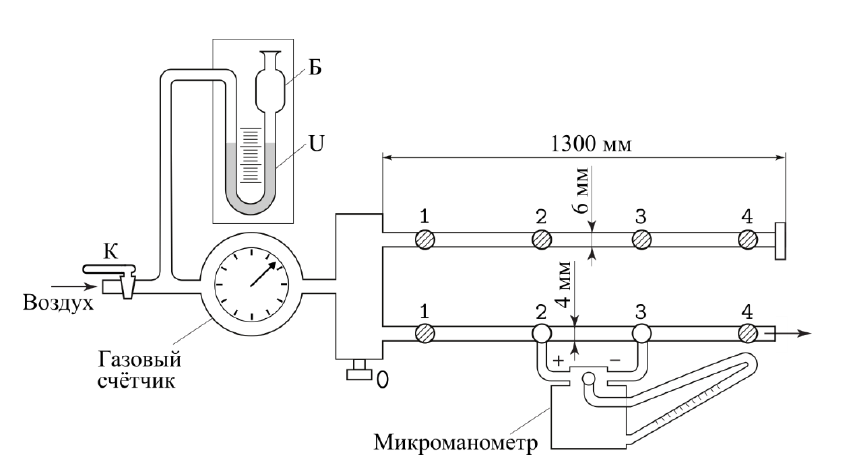
\includegraphics[scale=0.8]{lab133ris1.png}}
\caption{\textit{Схема установки}}
\end{figure}

Схема экспериментальной установки изображена на Рис. 1. Поток воздуха под давлением, немного превышающим атмосферное, поступает через газовый счётчик в тонкие металлические трубки. Воздух нагнетается
компрессором, интенсивность его подачи регулируется краном К. Трубки снабжены съёмными заглушками на концах. В рабочем состоянии открыта заглушка на одной (рабочей) трубке, микроманометр подключён к двум её выводам, а все остальные отверстия плотно закрыты пробками. Перед входом в газовый счётчик установлен водяной U-образный манометр. Он предохраняет счётчик от выхода из строя. При превышении максимального избыточного давления на входе счётчика (30 см вод.ст.) вода выплёскивается из трубки в защитный баллон Б, создавая шум
и привлекая к себе внимание экспериментатора

\subsubsection*{Ход работы}

Измерим давление и температуру в комнате: $P = (992\pm2)\cdot10^2(Па)$, $t = 24^{\circ}C$. После успешных предварительных настройки и запуска произведем предварительные расчёты. 

Оценим расход $Q_{кр}$ и перепад давлений $\Delta P_{кр}$ для трубки $d_1=3,95\pm0,05(мм)$, при которых число Рейнольдса станет равным критическому $R_e \approx 10^3$. Для этого примем вязкость воздуха равной $\eta_{возд} \approx 2\cdot10^{-5} (Па\cdot с)$, а плотность оценим по уравнению состояния идеального газа, характерную скорость потока возьмем из формулы (3). Так же оценим длину установления. Получим:

\begin{equation}
	Q_{кр} \approx 0,1 (л/c), \, \Delta P_{кр} \approx 160 (Па), \, l_{уст} \approx 40 (см).
\end{equation}

Согласно паспорту манометра, одно его деление будет равняться $0,2 \cdot 9,8$ Па. С учетом этого для трубки $d_1$ начнем снимать зависимость перепада давления $\Delta P$ от объемного расхода Q. Результаты измерений отразим в таблице 1 приложения.

Погрешность измерения времени возьмем как удвоенную реакцию человека (старт - стоп), давления как цену деления манометра, объема как цену деления и по классу точности. 

Измерим распределение давления при максимально возможном объемном расходе для разных длин трубок. Результаты измерений отразим в таблице 2 приложения.

Аналогичные измерения проведем для трубки $d_2=5,1\pm0,05(мм)$. Результаты отразим в таблицах 3 и 4 приложения. Точки легли на прямую, не проходящую через начало координат. Это значит, что все они были сняты при турбулентном течении. 

Измерим зависимость $Q(R)$, результаты отразим в таблице 5 приложения. Из них определим тип зависимости. Согласно теории, при турблунетном течении $Q\mathtt{\sim}R^4$. Действительно, построив график в логарифмических координатах, из наклона прямой вычисляется показатель истинной зависимости, который приблизительно равен 4.

\subsubsection*{Приложение}

\begin{table}[hbt]
\centering
\caption{\textit{Зависимость перепада давления от объемного расхода для первой трубки $d_1$}}
\scalebox{0.9}{
\begin{tabular}{|c|c|c|c|c|c|}
\hline
\textbf{$\Delta t,   c$} & \textbf{$\sigma_t, c$} & \textbf{$\Delta P, Па$} & \textbf{$\sigma_p, Па$} & \textbf{$\Delta V, л$} & \textbf{$\sigma_V, л$} \\ \hline
90                       & 1                      & 31                      & 3                       & 2                      & 0,1 \\ \hline
116                      & 1                      & 57                      & 4                       & 4                      & 0,1 \\ \hline
116                      & 1                      & 71                      & 5                       & 5                      & 0,1                   \\ \hline
108                      & 1                      & 92                      & 6                       & 6                      & 0,2 \\ \hline
112                      & 1                      & 118                     & 7                       & 8                      & 0,2 \\ \hline
108                      & 1                      & 139                     & 9                       & 9                      & 0,3                   \\ \hline
\multicolumn{6}{|c|}{\textbf{граница турбулентного и ламинарного течений}}                                                                              \\ \hline
110                      & 1                      & 155                     & 9                       & 10                     & 0,3                    \\ \hline
98                       & 1                      & 184                     & 11                      & 9                      & 0,3 \\ \hline
100                      & 1                      & 225                     & 14                      & 11                     & 0,3 \\ \hline
107                      & 1                      & 255                     & 15                      & 12                     & 0,4 \\ \hline
102                      & 1                      & 290                     & 18                      & 12                     & 0,4                   \\ \hline
98                       & 1                      & 321                     & 19                      & 12                     & 0,4 \\ \hline
94                       & 1                      & 365                     & 22                      & 12                     & 0,4                   \\ \hline
\end{tabular}
}
\end{table}

\begin{table}[]
\centering
\caption{\textit{Зависимость перепада давления от объемного расхода для второй трубки $d_2$}}
\scalebox{0.9}{
\begin{tabular}{|c|c|c|c|c|c|}
\hline
\textbf{$\Delta t,   c$} & \textbf{$\sigma_t, c$} & \textbf{$\Delta P, Па$} & \textbf{$\sigma_p, Па$} & \textbf{$\Delta V, л$} & \textbf{$\sigma_V, л$} \\ \hline
104                      & 1                      & 27                      & 3                       & 3                      & 0,1                    \\ \hline
107                      & 1                      & 37                      & 3                       & 4                      & 0,1                    \\ \hline
99                       & 1                      & 59                      & 4                       & 4                      & 0,1                    \\ \hline
103                      & 1                      & 69                      & 5                       & 5                      & 0,2                    \\ \hline
113                      & 1                      & 80                      & 5                       & 6                      & 0,2                    \\ \hline
116                      & 1                      & 96                      & 6                       & 7                      & 0,2                    \\ \hline
109                      & 1                      & 122                     & 8                       & 8                      & 0,2                    \\ \hline
\multicolumn{6}{|c|}{\textbf{граница турбулентного и ламинарного течений}}                                                                              \\ \hline
104                      & 1                      & 147                     & 9                       & 9                      & 0,3                    \\ \hline
113                      & 1                      & 176                     & 11                      & 11                     & 0,3                    \\ \hline
107                      & 1                      & 210                     & 13                      & 12                     & 0,4                    \\ \hline
100                      & 1                      & 274                     & 17                      & 12                     & 0,4                    \\ \hline
98                       & 1                      & 314                     & 19                      & 12                     & 0,4                    \\ \hline
112                      & 1                      & 353                     & 21                      & 16                     & 0,5                    \\ \hline
103                      & 1                      & 392                     & 24                      & 17                     & 0,5                    \\ \hline
\end{tabular}
}
\end{table}

\begin{table}[]
\centering
\caption{\textit{Зависимость перепада давления от длины первой трубки $d_1$}}
\begin{tabular}{|c|c|c|c|}
\hline
\textbf{$L, см$} & \textbf{$\sigma_L, см$} & \textbf{$\Delta P, Па$} & \textbf{$\sigma_P, Па$} \\ \hline
130,5            & 0,5                     & 451                     & 29                       \\ \hline
90,5             & 0,5                     & 314                     & 20                       \\ \hline
40,5             & 0,5                     & 186                     & 12                       \\ \hline
10,5             & 0,5                     & 90                      & 6                       \\ \hline
\end{tabular}
\end{table}

\begin{table}[]
\centering
\caption{\textit{Зависимость перепада давления от длины второй трубки $d_2$}}
\begin{tabular}{|c|c|c|c|}
\hline
\textbf{$L, см$} & \textbf{$\sigma_L, см$} & \textbf{$\Delta P, Па$} & \textbf{$\sigma_P, Па$} \\ \hline
130,5            & 0,5                     & 305 & 20                       \\ \hline
80,5             & 0,5                     & 219 & 14                       \\ \hline
40,5             & 0,5                     & 152 & 10                       \\ \hline
10,5             & 0,5                     & 85 & 6                       \\ \hline
\end{tabular}
\end{table}

\begin{table}[hbt]
\centering
\caption{\textit{Величина расхода для разных трубок при турбулентном течении}}
\begin{tabular}{|c|c|c|c|}
\hline
\textbf{$d, мм$}                         & 5,1    & 5,05   & 3,95   \\ \hline
\textbf{$\sigma_{d}, мм$}                & 0,05   & 0,05   & 0,1    \\ \hline
\textbf{$Q, л/с$}                        & 0,1025 & 0,0935 & 0,0272 \\ \hline
\textbf{$\sigma_{Q}, л/c \cdot 10^{-4}$} & 22,92  & 20,91  & 6,08   \\ \hline
\end{tabular}
\end{table}


\begin{figure}[hbt]
\center{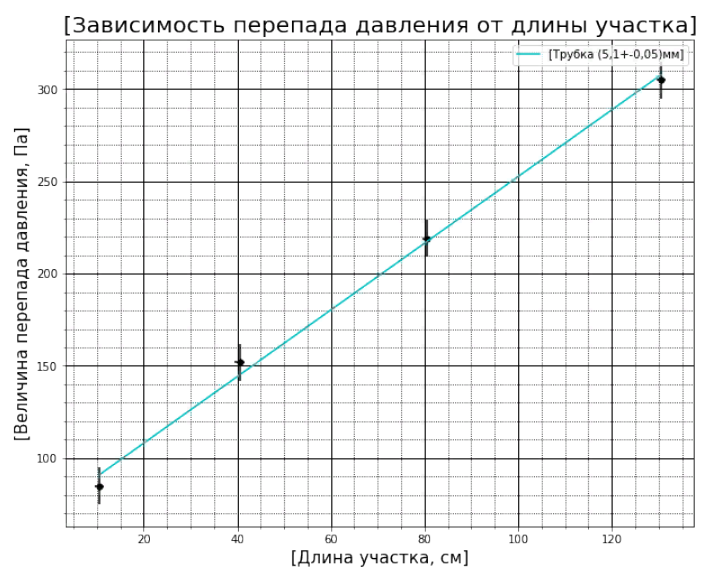
\includegraphics[scale=0.8]{lab133ris5.png}}
\caption{\textit{Зависимость перепада давления от длины участка на $d_1$}}
\end{figure}

\begin{figure}[hbt]
\center{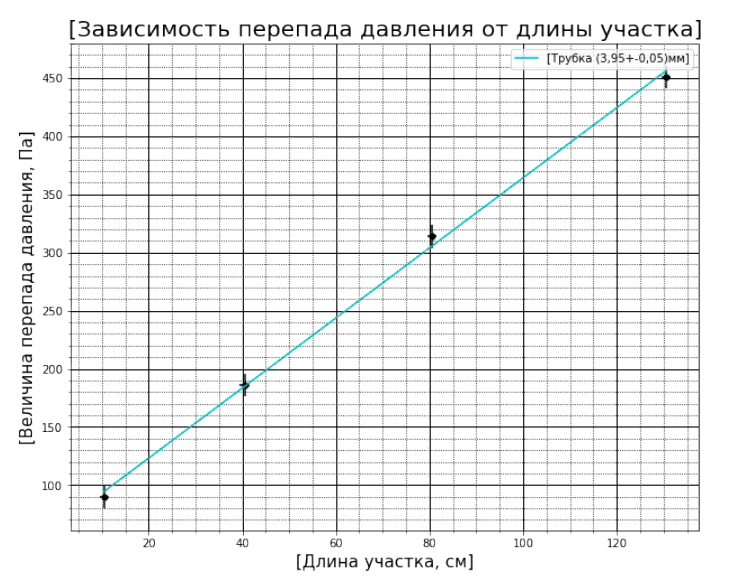
\includegraphics[scale=0.8]{lab133ris6.png}}
\caption{\textit{Зависимость перепада давления от длины участка на $d_2$}}
\end{figure}

\begin{figure}[hbt]
\center{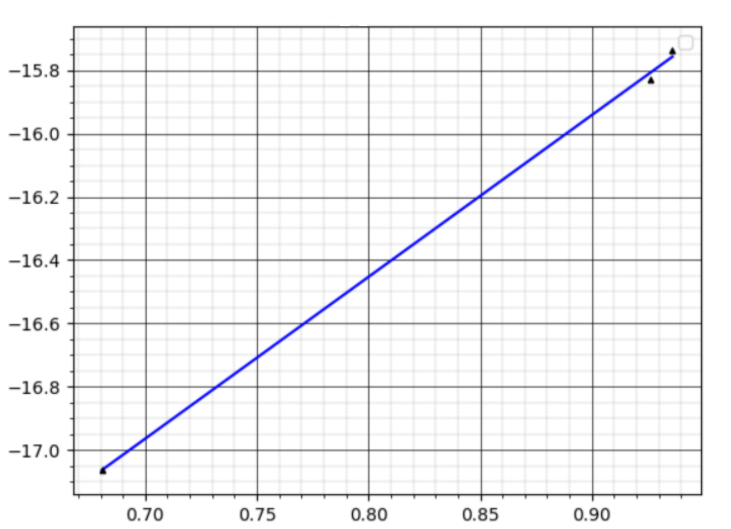
\includegraphics[scale=0.8]{lab133ris7.png}}
\caption{\textit{Зависимость расхода от диаметра трубки в логарифмических координатах}}
\end{figure}

\end{document}